\documentclass{beamer}
\mode<presentation>
{
  \usetheme{default}      % or try Darmstadt, Madrid, Warsaw, ...
  \usecolortheme{default} % or try albatross, beaver, crane, ...
  \usefonttheme{default}  % or try serif, structurebold, ...
  \setbeamertemplate{navigation symbols}{}
  \setbeamertemplate{caption}[numbered]
} 

\usepackage[english]{babel}
\usepackage[utf8x]{inputenc}
\usepackage{scrextend}
\usepackage{graphicx}
\usepackage{booktabs}
\usepackage{adjustbox}
\usepackage{marvosym}
\graphicspath{ {E:/faculta/Conf/ppt/images/} }

\title[Pres]{Identifying logical dependencies from co-changing classes}
\author{Stana Adelina Diana}
\institute{Department of Computer and Information Technology\\
Politehnica University Timisoara, Romania}
\date{May, 2019}

\begin{document}

\begin{frame}
  \titlepage
\end{frame}

% Uncomment these lines for an automatically generated outline.
%\begin{frame}{Outline}
%  \tableofcontents
%\end{frame}
%%%%%%%%%%%%%%%%%%%%%%%%%%%%%%%%%%%%%%%%%%
 \begin{frame}
\frametitle{Dependencies}
\begin{columns}
\begin{column}{0.5\textwidth}
    \begin{center}
     \begin{figure}
	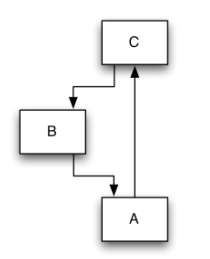
\includegraphics[width=\textwidth]{depend.PNG}
	\caption{\label{fig:your-figure}Dependencies in a project}
     \end{figure}
     \end{center}
\end{column}
\begin{column}{0.5\textwidth}

A  \texttt{dependency} is a relationship that shows that an element, or set of elements, requires other elements for their specification or implementation. [ UML Specification]

\end{column}
\end{columns}
\end{frame}
%%%%%%%%%%%%%%%%%%%%%%%%%%%%%%%%%%%%%%%%%%

 \begin{frame}
\frametitle{Structural dependencies}
\begin{block}{Definition}
Structural dependencies are the result of \it{source code analysis} and can be extracted from : members, call parameters, local variables. 
\end{block}

\begin{center}
     \begin{figure}
	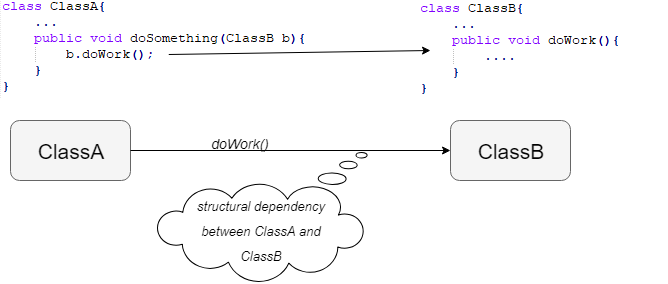
\includegraphics[width=\textwidth]{structural_dep.png}
	\caption{\label{fig:fig}Example of structural dependency between two classes}
     \end{figure}
\end{center}

\end{frame}

%%%%%%%%%%%%%%%%%%%%%%%%%%%%%%%%%%%%%%%%%%%

 \begin{frame}
\frametitle{Logical dependencies}
\begin{block}{Definition}
 Logical dependencies are the result of software history analysis and can reveal relationships that are not present in the source code code (structural dependencies).
\end{block}

\begin{center}
     \begin{figure}
	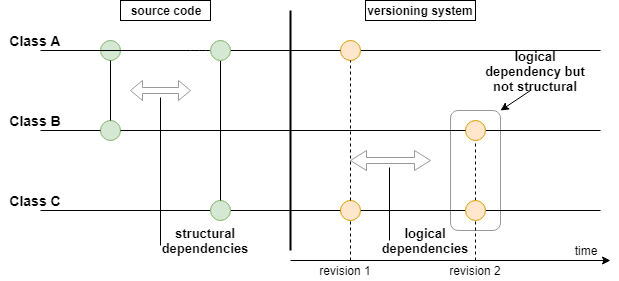
\includegraphics[width=\textwidth]{fig1.png}
	\caption{\label{fig:fig1}Example of logical and structural dependencies}
     \end{figure}
\end{center}

\end{frame}

%%%%%%%%%%%%%%%%%%%%%%%%%%%%%%%%%%%%%%%%%%%
\begin{frame}
\frametitle{Logical dependencies}
\begin{block}{Research questions}
 \vskip 0.3cm 
We build logical dependencies based on the following questions :\\
 \textit{\textbf{Question 1:} Which is the most frequent size for a commit transaction ?}\\
 \textit{\textbf{Question 2:} Is it necessary to set a threshold on the size of commit transactions which are considered to generate valid logical dependencies ?}\\
 \textit{\textbf{Question 3:} Considering changes which are only in comments as valid can lead to additional logical dependencies ?}\\
 \textit{\textbf{Question 4:} How many occurrences of a logical dependency are needed to consider it a valid logical dependency ? }\\ 
 \textit{\textbf{Question 5:} How does filtering affect the overlap between structural and logical dependencies ?}
\end{block} 
\end{frame}

%%%%%%%%%%%%%%%%%%%%%%%%%%%%%%%%%%%%%%%%%%%

 \begin{frame}
\frametitle{Logical dependencies}
\begin{center}
     \begin{figure}
	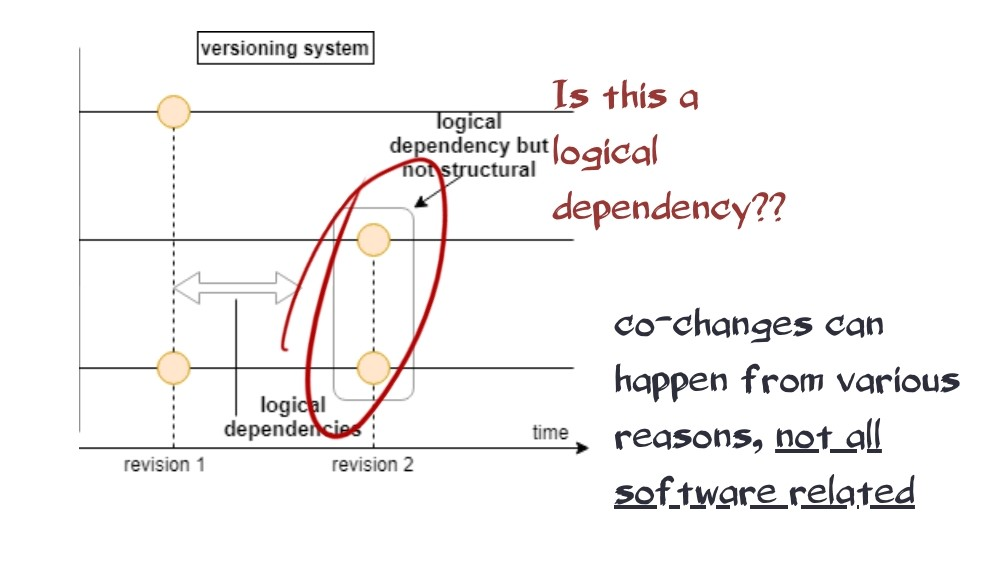
\includegraphics[width=\textwidth]{co-change.jpg}
	%\caption{\label{fig:fig1}Logical dependencies and co-changing classes}
     \end{figure}
\end{center}

\end{frame}

%%%%%%%%%%%%%%%%%%%%%%%%%%%%%%%%%%%%%%%%%%%

\begin{frame}
\frametitle{Co-changing classes}
\vskip 0.2cm
\begin{center}
     \begin{figure}
	
\includegraphics[width=\textwidth]{compare.jpg}
	%\caption{\label{fig:fig1}Logical dependencies and co-changing classes}
     \end{figure}
\end{center}

\end{frame}

%%%%%%%%%%%%%%%%%%%%%%%%%%%%%%%%%%%%%%%%%%%

 \begin{frame}
\frametitle{Filter co-changing classes, how?}
\vskip 0.2cm
\begin{center}
     \begin{figure}
	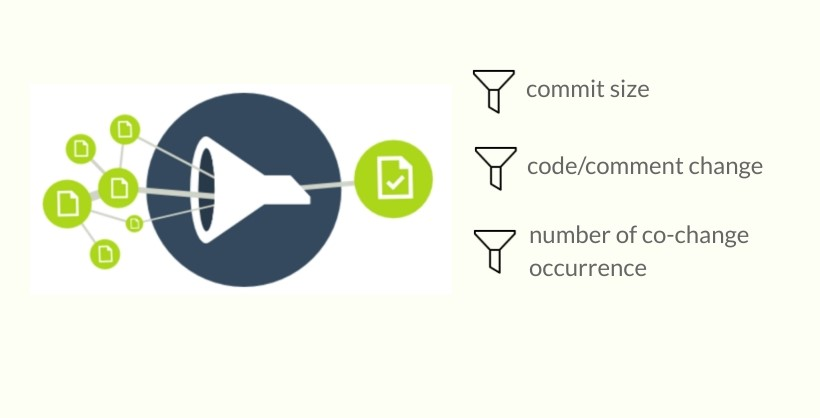
\includegraphics[width=\textwidth]{filter.jpg}
	%\caption{\label{fig:fig1}Logical dependencies and co-changing classes}
     \end{figure}
\end{center}

\end{frame}


 \begin{frame}
\frametitle{Commit transaction size}
\vskip 0.2cm
\begin{center}
     \begin{figure}
	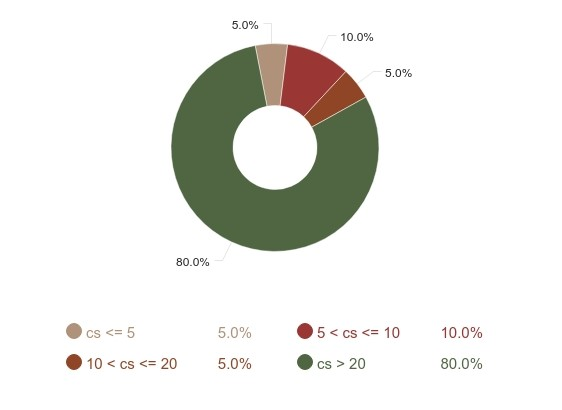
\includegraphics[width=\textwidth]{cs_size.jpg}
	%\caption{\label{fig:fig1}Logical dependencies and co-changing classes}
     \end{figure}
\end{center}

\end{frame}

%%%%%%%%%%%%%%%%%%%%%%%%%%%%%%%%%%%%%%%%%%%

 \begin{frame}
\frametitle{Conclusions}
 \begin{itemize}
        \item  Large number of structural dependencies are not doubled by logical \MVRightarrow{} systems partially stable
        \item  + -3\% for comments as a change
        \item The number of changed files taken into consideration influence the results
	\begin{itemize}   
	\item big threshold  \MVRightarrow{} not so relevant logical dependencies
	\item small threshold (5~10)  \MVRightarrow{} more accurate results
    	\end{itemize}
      \item Filtering the logical dependencies after occurrences is good only for projects with a significant number of commits. 
    \end{itemize}
\begin{block}{Future work}
Investigate the cause for the large number of logical dependencies which are not overlapping with structural dependencies.
\end{block}
\end{frame}

%%%%%%%%%%%%%%%%%%%%%%%%%%%%%%%%%%%%%%%%%%%

\end{document}
